\begin{frame}
	\frametitle{Aplicaciones Similares}
	\begin{columns}
		\begin{column}{0.6\textwidth}
			\block{\it Remind}
				\begin{itemize}
					\item Forma sencilla de enviar mensajes a estudiantes y padres.
					\item Los profesores, monitores o administradores pueden enviar recordatorios, deberes o mensajes motivadores.
					\item Seguro, teléfonos confidenciales.
					\item Los profesores pueden enviar anuncios o mensajes tipo chat.
				\end{itemize}
			\endblock{}
		\end{column}
		\begin{column}{0.4\textwidth}
			\hfill 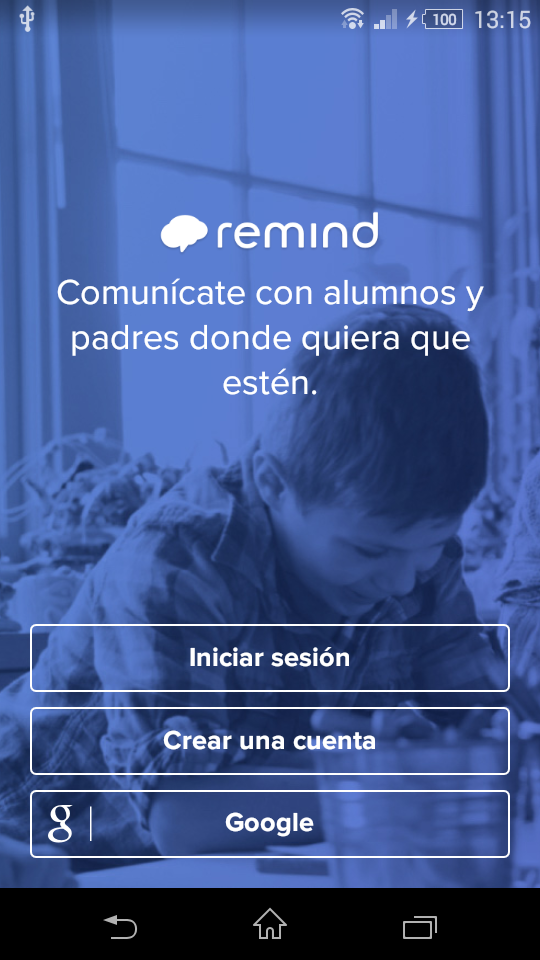
\includegraphics[width=0.7\linewidth]{Images/Remind.png}
		\end{column}
	\end{columns}
\end{frame}

%------------------------------------------------------------------

\begin{frame}
	\frametitle{Aplicaciones Similares}
	\begin{columns}
		\begin{column}{0.6\textwidth}
			\block{\it miColegioApp}
			\begin{itemize}
				\item El colegio contrata los servicios.
				\item Registro de usuarios.
				\item Introducir el código del centro en la aplicación.
				\item Se asocian a los usuarios con un centro.
				\item Los usuarios pueden recibir notificaciones, circulares y boletines.
			\end{itemize}
			\endblock{}
		\end{column}
		\begin{column}{0.4\textwidth}
			\hfill 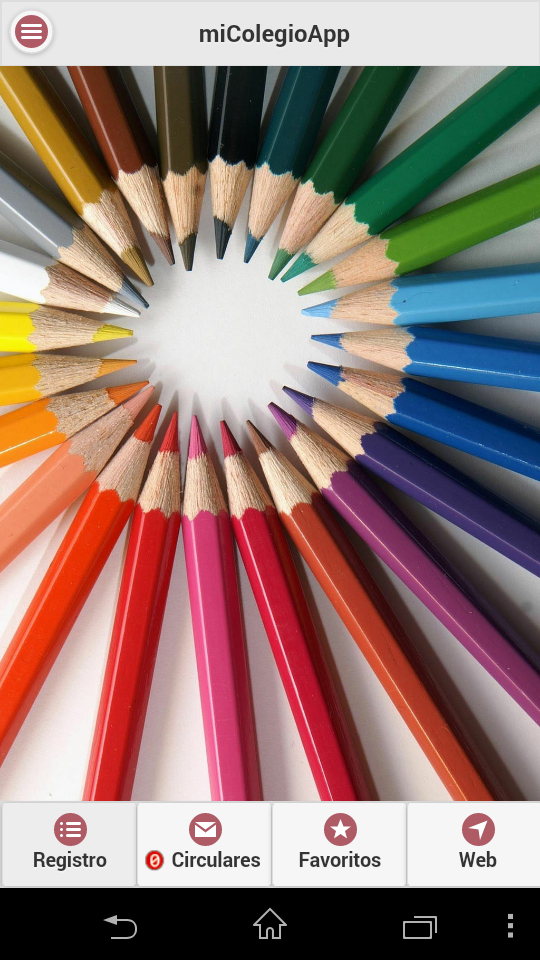
\includegraphics[width=0.7\linewidth]{Images/miColegioApp.png}
		\end{column}
	\end{columns}
\end{frame}

%------------------------------------------------------------------
\begin{frame}
	\frametitle{Descripción}
	\block{Definición de términos}
		\begin{itemize}
			\item {\it Activity}.
			\item {\it Fragment}.
			\item {\it Dialog}.
		\end{itemize}
	\endblock{}
	
	{\usebeamercolor[fg]{titlegraphic}\inserttitlegraphic\par}
	\vfill 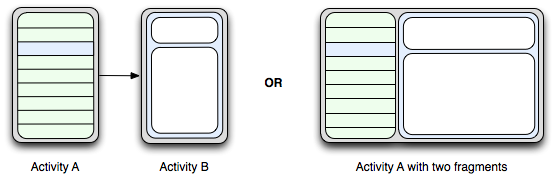
\includegraphics[width=0.7\linewidth]{Images/android_fragments}
	\hfill 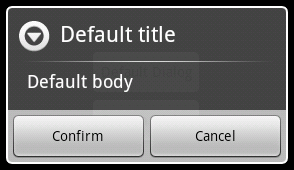
\includegraphics[width=0.25\linewidth]{Images/dialog}
	
\end{frame}

%------------------------------------------------------------------

%Estilo de este frame portrait (hoja normal posición de folio)
\begin{frame}
	\frametitle{Descripción}
	\begin{center}
		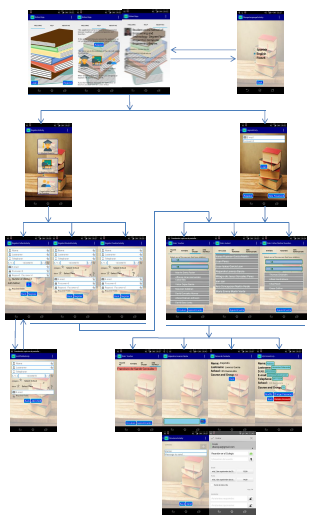
\includegraphics[width=0.3\linewidth]{Images/mapaActividades.png}
	\end{center}
\end{frame}

%------------------------------------------------------------------

\begin{frame}
	\frametitle{Descripción}
	\block{}
		Vídeo ilustrativo del funcionamiento de la aplicación.
	\endblock{}
\end{frame}